\section{LP21 Absorption et émission de la lumière (Martin)}

\begin{header}
\begin{tabular}{p{0.4\textwidth} l}
\niveau & \prerequis \\
CPGE    & \textbullet{} Corps noir \\
        & \textbullet{} Optique ondulatoire \\
        & \textbullet{} Modèle de l’électron élastiquement lié \\
        & \textbullet{} Distribution de Boltzmann \\
        & \textbullet{} Mécanique quantique : quantification de l'énergie
\end{tabular}

\noindent
\objectif
Expliquer les intéraction matière rayonnement avec les résultats de la mécanique quantique.
\end{header}

{
\paragraph{Bibliographie :}
\begin{itemize}
\item 
\end{itemize}
}

\subsection{Introduction}

\begin{slide}
\textbf{Les limites du modèle.}
\end{slide}

Le modèle de l'électron  élastiquement lié permet d'expliquer les spectres d'absorption, comme celui du Soleil.
Il ne permet cependant pas d'expliquer les spectres d'émission de composés simples comme celui d'une lampe à vapeur de mercure.
Il faut donc un nouveau modèle pour décrire ces spectres.

\subsection{Les phénomènes d'absorption et d'émission}

\subsubsection{Position du problème (1'30)}

La solution a été proposée par Albert Einstein en 1917 avec un modèle phénoménologique.

\begin{slide}
\textbf{Le modèle d'Einstein.}
\end{slide}

On veut décrire l'interaction entre la lumière et la matière.
Pour cela, on considère :
\begin{itemize}
\item la matière comme un ensemble d'atomes assimilés à des systèmes à deux niveaux ($E_1$ pour le fondamental et $E_2$ pour l'état excité) ;
\item la lumière comme un flux de photons caractérisés par leur énergie $E = h\nu$.
\end{itemize}
Pour qu'il y ai interaction, il faut que le rayonnement soit résonant avec la transition atomique soit $E_2 - E_1 = h\nu_0$.

On pose $u(\nu)$ la densité spectrale volumique d'énergie électromagnétique, caractéristique du rayonnement.
Pour décrire l'état de la matière, on va s'intéresser à $N_i$ le nombre d'atomes par unité de volume et d'énergie $E_i$.
En supposant que cette densité est très grande, on peut utiliser un modèle statistique pour décrire cette assemblée d'atomes.
Les niveaux d'énergie ne sont pas infiniment fins, ce qui impose de prendre en compte le profil spectral normé de la transition $g(\nu)$ tel que :
\begin{equation}
\int_0^\infty g(\nu)d\nu = 1.
\end{equation}

\begin{transition}
On va maintenant décrire les différents processus associés à l'absorption et l'émission de la lumière responsables de transitions atomiques.
\end{transition}

\subsubsection{Les coefficients d'Einstein (4'30)}

On remplit progressivement le tableau :
\begin{table}[!h]
\center
\begin{tabular}{c|c|c}
Émission spontanée & Absorption & Émission stimulée \\
\hline \hline \\
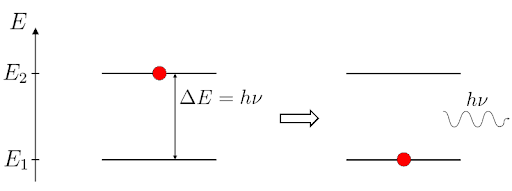
\includegraphics[height=50pt]{Lecons_de_physique_2019-2020/Lecons_autres/emission_spontanee.png} & 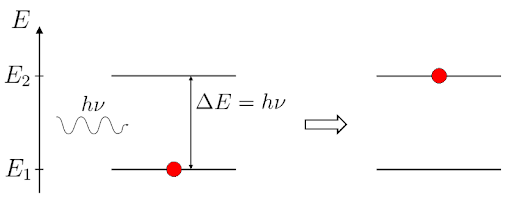
\includegraphics[height=50pt]{Lecons_de_physique_2019-2020/Lecons_autres/absorption.png} & 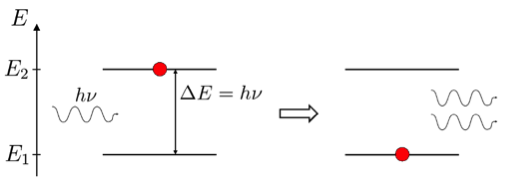
\includegraphics[height=50pt]{Lecons_de_physique_2019-2020/Lecons_autres/emission_stimulee.png} \\
$\left(\frac{\d N_2}{\d t}\right)_\mathrm{sp} = -A_{21} N_2$ & $\left(\frac{\d N_2}{\d t}\right)_\mathrm{ab} = B_{12} N_1 u(\nu_0)$ & $\left(\frac{\d N_2}{\d t}\right)_\mathrm{st} = -B_{21} N_2 u(\nu_0)$ \\
$[A_{21}] = \second^{-1}$ & $[B_{12}] = \meter^3\joule^{-1}\second^{-1}$ & $[B_{21}] = \meter^3\joule^{-1}\second^{-1}$ \\
Dir, pola, phase aléatoire & & Dir, pola, phase identique \\
						   & & au photon incident 
\end{tabular}
\end{table}

Ici on suppose que l'on est dans le cas d'un spectre large bande, c'est à dire que le profil de la densité spectrale d'énergie $u$ est large devant le profil de raie $g$ (schéma).
On peut alors faire l'approximation
\begin{equation}
\int_0^\infty u(\nu) g(\nu) \d \nu \approx u(\nu_0).
\end{equation}

\begin{slide}
\textbf{Émission spontanée.}
\end{slide}

\begin{experience}
\textbf{Mesure des longueurs d'onde émises par une lampe à vapeur de mercure au goniomètre.}
On montre les raies de la lampe à vapeur de mercure d'abord qualitativement avec le prisme puis on mesure l'angle au minimum de déviation sur le goniomètre avec le réseau à 600 traits par mm.
On compare pour les trois raies les plus intenses (il y a le doublet jaune donc quatre raies au total).
\end{experience}

Ce type d'étude spectrale permet d'identifier les gaz par leur empreinte digitale spectrale.

\begin{experience}
\textbf{Spectre d'absorption de la rhodamine dans l'éthanol.}
\end{experience}

L'émission stimulée apparait symétriquement à l'absorption (stimulée).
Grâce à l'émission stimulée on peut obtenir de la lumière cohérente utile pour faire des interférences par exemple.

\begin{transition}
L'émission stimulée est toutefois difficile à observer.
Avant de poursuivre on souhaite vérifier que les processus décrits par Einstein sont cohérents avec les observations expérimentales.
\end{transition}

\subsection{Mise à l'épreuve du modèle}

\subsubsection{Bilan à l'équilibre thermique (16')}

On veut confronter le modèle à des observations expérimentales étudiées à l'époque : celles associées au spectre d'émission du corps noir.
La variation temporelle de population du niveau excité peut s'exprimer en fonction des différents processus de transition évoqués précédemment :
\begin{equation}
\frac{\d N_2}{\d t} = -A_{21} N_2 - B_{21} N_2 u(\nu) + B_{12} N_1 u(\nu).
\end{equation}
En régime permanent, cette variation est nulle ce qui permet d'exprimer la densité spectrale d'énergie :
\begin{equation}
u(\nu) = \frac{A_{21}}{B_{21}}\frac{1}{\frac{B_{12}}{B_{21}}\frac{N_1}{N_2} - 1}.
\end{equation}
A l'équilibre thermodynamique, le rapport des populations entre les niveaux fondamental et excité s'exprime en fonction du facteur de Boltzmann, si bien que
\begin{equation}
\frac{N_1}{N_2} = e^{\frac{E_2-E_1}{k_B T}} = e^{\frac{h\nu}{k_B T}}.
\end{equation}
On en déduit
\begin{equation}
u(\nu) = \frac{A_{21}}{B_{21}} \frac{1}{\frac{B_{12}}{B_{21}} e^{\frac{h\nu}{k_B T}} - 1}.
\end{equation}

Les résultats obtenus par Planck donnent une expression similaire
\begin{equation}
u(\nu) = \frac{8\pi\nu^3}{c^3} \frac{1}{e^{\frac{h\nu}{k_B T}} - 1}.
\end{equation}
En posant $B_{12} = B_{21} = B$ et
\begin{equation}
\frac{A_{21}}{B_{21}} = \frac{8\pi\nu^3}{c^3},
\end{equation}
l'expression de Planck et celle d'Einstein donnent le même résultat.

\begin{slide}
\textbf{Le modèle d'Einstein (bis).}
\end{slide}

L'émission stimulée est bel et bien nécessaire pour retrouver le spectre du corps noir.

\begin{transition}
On veut maintenant comparer l'importance relative des processus d'émission spontanée et stimulée.
\end{transition}

\subsubsection{Comparaison des processus (22')}

En utilisant l'expression de $u$ trouvée dans le cas du corps noir, on peut exprimer le rapport $\alpha$ entre les taux de désexcitation liés à l'émission stimulée et l'émission spontanée sous la forme
\begin{equation}
\alpha = \frac{\left(\frac{\d N_2}{\d t}\right)_\mathrm{st}}{\left(\frac{\d N_2}{\d t}\right)_\mathrm{sp}} = \frac{1}{e^{\frac{h\nu}{k_B T}} - 1}.
\end{equation}

\begin{slide}
\textbf{Le modèle d'Einstein (bis, suite).}
\end{slide}

On peut estimer ce coefficient pour quelques cas particuliers :
\begin{itemize}
\item à $T=\unit{300}{\kelvin}$ et pour $\lambda=\unit{600}{\nano\meter}$, $\alpha = 10^{-25}$ : l'émission spontanée prédomine largement ;
\item à $T=\unit{300}{\kelvin}$ et pour $\lambda > \unit{30}{\micro\meter}$, $\alpha > 1$ : l'émission stimulée joue un rôle important à partir du domaine microonde ;
\item à $T=\unit{5000}{\kelvin}$ et pour $\lambda=\unit{600}{\nano\meter}$, $\alpha = 10^{-2}$ : la lumière visible émise par le soleil est incohérente ;
\item à $T=\unit{35000}{\kelvin}$ et pour $\lambda=\unit{600}{\nano\meter}$, $\alpha = 1$ : l'émission stimulée devient importante aux très hautes températures.
\end{itemize}

\begin{transition}
Dans la vie courante il est donc impossible d'observer d'émission stimulée.
Il faut pour cela se placer hors de l'équilibre thermodynamique.
\end{transition}

\subsection{Application au laser}

\subsubsection{Amplification (26')}

On fait un bilan d'énergie entre $t$ et $t+\d t$ sur un volume de section $S$ compris entre $z$ et $z+\d z$.
Les variations d'énergie de ce volume sont dues aux flux d'énergie décris par le vecteur de Poynting $\Pi$ et aux absorption et émission de photon par la matière.
Comme on s'intéresse à un milieu amplificateur, on peut supposer la densité spectrale d'énergie très grande si bien que l'émission spontanée devient négligeable devant l'émission stimulée.
On a alors
\begin{equation}
\left(\frac{\d u}{\d t}\right) S\d z \d t = (\Pi(z) - \Pi(z+\d z))S \d t - \left[ \left(\frac{\d N_2}{\d t}\right)_\mathrm{st} + \left(\frac{\d N_2}{\d t}\right)_\mathrm{ab} \right] h\nu S \d z \d t.
\end{equation}
Comme $u(\nu) = \Pi/c$ et en régime permanent, on obtient
\begin{equation}
\frac{\d\Pi}{\d z} = \frac{Bh\nu}{c}(N_2-N_1)\Pi.
\end{equation}
On  obtient donc une amplification si $N_2>N_1$, c'est à dire si on a une inversion de population.
Cette inversion de population est permise grâce à un processus de pompage.

\begin{transition}
Ici on peut amplifier une lumière mais la source ainsi obtenue n'est pas vraiment cohérente car les photons incidents qui déclenchent l'émission stimulée sont incohérents.
\end{transition}

\subsubsection{Le laser (34')}

Pour obtenir une véritable source cohérente, il faut appliquer une rétroaction, c'est à dire boucler le système à l'aide d'une cavité Fabry-Perot (schéma d'une cavité avec un milieu amplificateur).
On obtient alors l'équation d'évolution pour $\Pi$
\begin{equation}
\frac{\partial \Pi}{\partial z} = (\gamma(\nu) - \beta ) \Pi,
\end{equation}
où
\begin{equation}
\gamma(\nu) = \frac{Bh\nu}{c}(N_2-N_1)
\end{equation}
est le gain associé au milieu amplificateur et $\beta$ est lié aux pertes.
Pour obtenir l'effet laser, il faut $\gamma(\nu) > \beta$, ce qui peut se représenter graphiquement.
On représente alors sur un même graphique les courbes de gain (une courbe en cloche large spectralement), de pertes (constantes), ce qui permet de donner la plage de fonctionnement du laser.

Il faut aussi tenir compte des résonances de la cavité Fabry-Perot, que l'on représente sur le graphique et qui limite les fréquences accessibles avec le laser.
On obtient ainsi un faisceau cohérent temporellement et spatialement.

\begin{experience}
\textbf{Mise en évidence de la cohérence spatiale d'un faisceau laser avec le speckle.}
\end{experience}

\begin{slide}
\textbf{Laser.}
L'effet laser a d'abord été obtenu dans le domaine microonde avec le maser puis dans le domaine visible avec un laser à rubis.
\end{slide}

\begin{slide}
\textbf{Laser (bis).}
Il existe un vaste zoologie de lasers.
\end{slide}

\subsection{Conclusion (38')}

Albert Einstein a développé un nouveau modèle pour expliquer l'interaction rayonnement matière.
Ouverture sur différentes applications du laser : blu-ray, chirurgie, GPS, génération de deuxième harmonique, etc.

\begin{slide}
\textbf{Applications.}
\end{slide}